The simplest process allowing to set constraints on EFT operators is Drell-Yan di-lepton and lepton-neutrino production at high invariant mass, for concreteness we focus on oblique corrections only, generalizations being rather obvious. These corrections can be parametrized in the electroweak sector by the four oblique parameters $S$, $T$, $W$ and $Y$. These correspond to four operators that modify the propagators of the $W$ and $Z$ bosons both on the pole ($S$ and $T$) and off the pole, i.e.~on the tails ($W$ and $Y$). Hadron colliders can hardly compete with lepton colliders for pole observable. However, due to the enhancement of the kinematic distributions with respect to the corresponding SM ones at high energy, hadron colliders are particularly suited to study off-pole observables like $W$ and $Y$. Deviations from the SM proportional to $W$ and $Y$ can be parametrized through the two operators from table~\ref{tab:dim6ops},
\begin{equation}
 -\frac{W}{2m_W^2}\mathcal{O}_{2W}   \,, \quad  -\frac{Y}{2m_W^2}\mathcal{O}_{2W}   
 \end{equation}
They modify the neutral and charged gauge boson propagators as
\begin{equation}\label{eq:propagators}
\begin{array}{ll}
& P_{\hspace{-1pt}{N}}\hspace{-1pt} = \hspace{-2.5pt}\left[\hspace{-2pt}
\begin{array}{cc}
 \frac{1}{q^2}-\frac{t^{2}{\rm{\sc{W}}}+{\rm{\sc{Y}}}}{m_Z^2} & \frac{t \left(\left({\rm{\sc{Y}}}+{\rm\hat{T}}\right) c^2+s^2 {\rm{\sc{W}}}-{\rm\hat{S}}\right)}{\left(c^2-s^2\right) \left(q^2-m_Z^2\right)}+\frac{t ({\rm{\sc{Y}}}-{\rm{\sc{W}}})}{m_Z^2} \\
 \star & \frac{1+ {\rm\hat{T}}-{\rm{\sc{W}}}-t^{2}{\rm{\sc{Y}}}}{q^2-m_Z^2}-\frac{t^{2}{\rm{\sc{Y}}}+{\rm{\sc{W}}}}{m_Z^2} \\
\end{array}
\hspace{-2pt}
\right] \\
& P_{\hspace{-1pt}{C}}\hspace{-1pt} =
\begin{array}{c}
\frac{1+\left( \left({\rm\hat{T}}-{\rm{\sc{W}}}-t^2 {\rm{\sc{Y}}}\right)-2 t^2 \left({\rm\hat{S}}-{\rm{\sc{W}}}-{\rm{\sc{Y}}}\right)\right)/(1-t^2)}{(q^{2}-m_W^2)}-\frac{{\rm{\sc{W}}}}{m_W^2}\,,
\end{array}
\end{array}
\end{equation}
Studying the tails of the invariant mass distribution of two leptons and of the transverse mass of lepton-neutrino, one can set constraints on these observables. For details on the procedure see ref.~\cite{Farina:2016rws}, also extended to dijet and multijet analyses in ref.s~\cite{Alioli:2017nzr,Alioli:2017jdo}. The prospect results for the HL-LHC and HE-LHC are shown in fig.~\ref{fig:DY-WY}
\begin{figure}[ht]
\centering
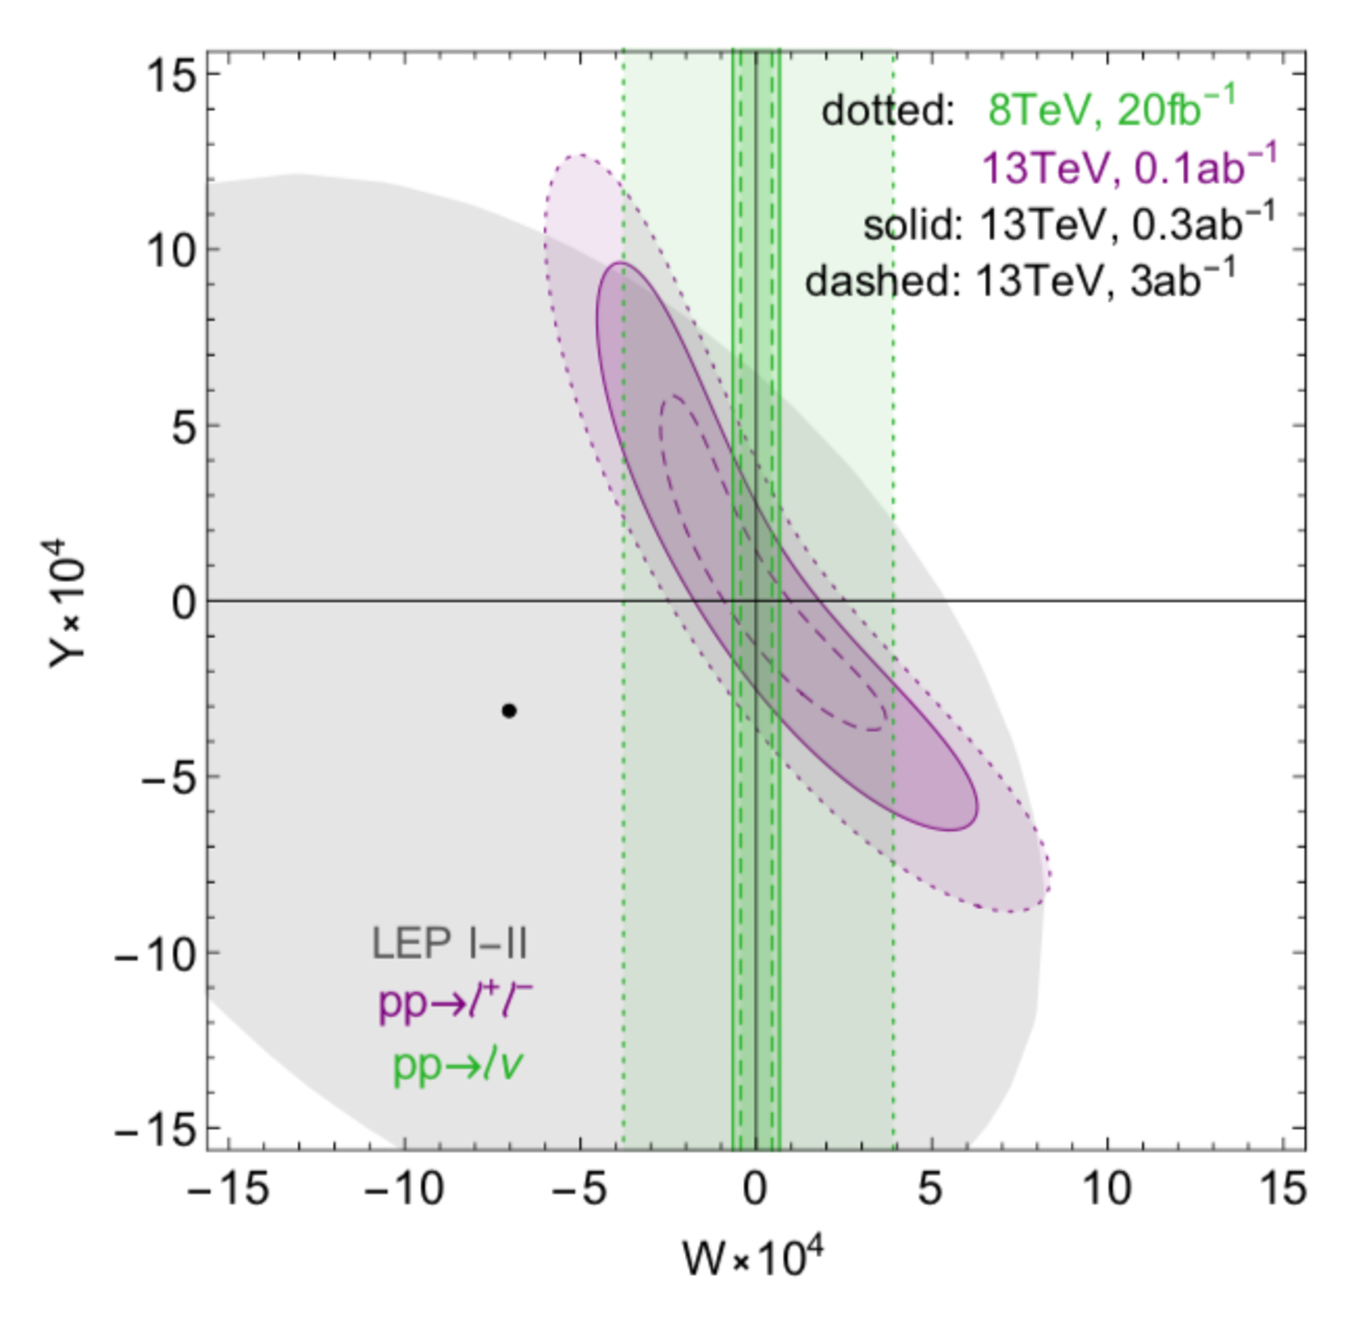
\includegraphics[width=0.49 \textwidth ]{\main/section4/plots/WY_HL-LHC}
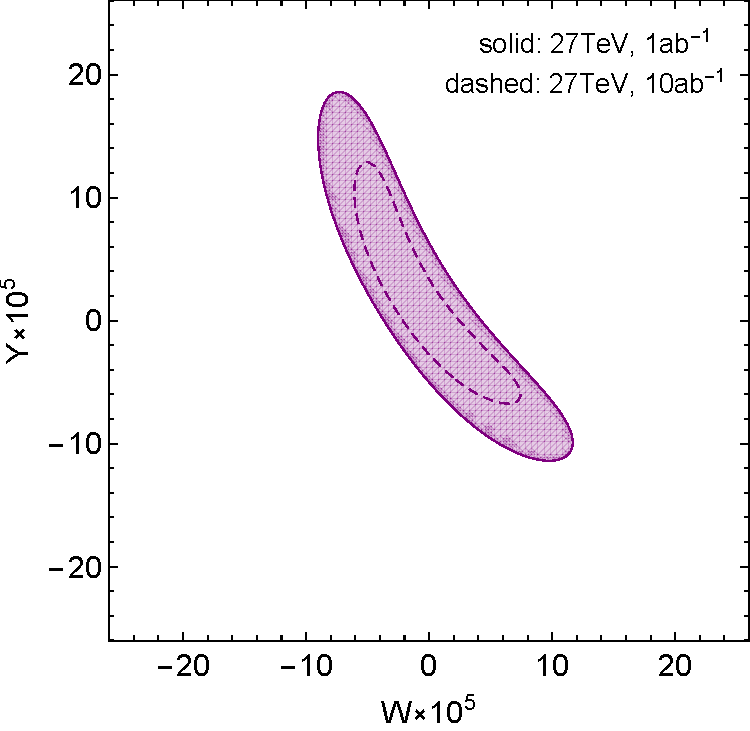
\includegraphics[width=0.468 \textwidth ]{\main/section4/plots/WY_HE-LHC}
\caption{Left: LHC and HL-LHC. Right: HE-LHC}
\label{fig:DY-WY}
\end{figure}
